\newpage
\section{Daten-Pipeline}
\subsection{Bilder aufnehmen}
Die Aufnahme der Bilder geschah unverändert mit Aparatur und C++ Code von Tabea Mendez welche aus Ihrer Masterarbeit entstand. 
Das Ergebnis waren jeweils 8 Bilder aus einer Situation. 
Eine Situation bestand aus 4 Kameras, wobei jede Kamera jeweils ein schwarzweiss-Bild mit UV-Beleuchtung und ein schwarzweiss-Bild mit normaler weisser Beleuchtung gemacht wurde.
Um später die Detektion von Fingern mithilfe  
Pro Durchgang konnten maximal 6000 Situationen aufgenommen werden, bevor der Arbeitsspeicher des dafür verwendeten Computers an seine Grenzen kam. 

Eine Verbesserung könnte hier erreicht werden, wenn man das Programm in 2 verschiedene Threads aufteilt.
Dabei ist ein Thread für das Aufnehmen der Daten und der andere für das abspeichern derselben zuständig.
So könnte \grqq{}unendlich lange\grqq{} Daten aufgenommen werden.
\subsection{Fingerdetektion}
\subsection{CSV generieren}
\subsection{Python-Objekt generieren}
%Label-Tensor
\begin{figure}	
	\centering
	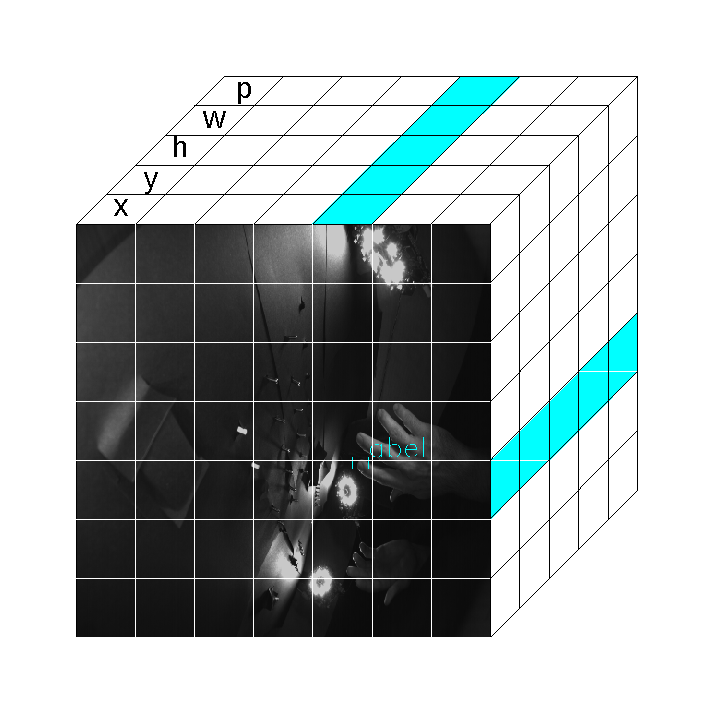
\includegraphics[width=.8\textwidth]{Kapitel/DatenPipeline/Bilder/LabelTensor.pdf}
	\caption{Label-Tensor}
	\label{img:label_tensor}
\end{figure} 
\subsection{Daten in Neuronales Netzwerk einlesen}

